\chapter{Effiziente Implementierungen}

%%% section %%%
\section{Langzahlen}

In (asymmetrischer) Kryptographie benötigen wir ülicherweise Werte, die weit größer sind, als die native Wortlänge der zugrundeliegenden Hardware.
Die meisten Register haben eine Wortlänge von 64 bit. Typische Schlüssellängen, beispielsweise für RSA Verschlüsselung, sind heutzutage 1024 bis 4096 bits.

\paragraph{Wie können solche Zahlen dargestellt werden?}

Eine Auswahl an Möglichkeiten ist:

\begin{enumerate}
    \item Residuen-Repräsentation \index{Residuen-Repräsentation}
    \item Verwendung von Arrays in nativer Wortgröße \index{Arrays mit nativer Wortgröße}
    \item Verwendung von Arrays kleiner als die native Wortgröße \index{Arrays kleiner als die native Wortgröße}
\end{enumerate}

\paragraph{Wie kann eine effiziente Modulo Reduktion implementiert werden?}

Die Division großer Zahlen ist sehr teuer, deswegen wurden Methoden für eine Restbestimmung ohne direkte Division entwickelt:

\begin{enumerate}
    \item Barrett Reduktion \index{Barrett Reduktion}
    \item Montgomery Arithmetik \index{Montgomery Arithmetik}
\end{enumerate}

\paragraph{Wie kann effizient Exponentiation implementiert werden}

Bei Square \& Multiply ist die Berechnung schneller, je weniger Bits des Exponenten den Wert \verb|1| haben, siehe NAF \index{NAF} (Non-adjacent Form) \index{NAF}.

%%% subsection %%%
\subsection{Residuen-Repräsentation} \index{Residuen-Repräsentation}

Wir wählen $r$ verschiedene koprime (paarweise teilerfremde) Moduli $m_1, \ldots, m_r$ und eine beliebige Zahl $x$. Wir können eine Darstellung

\begin{equation}
    x = (x_1, \ldots, x_r)
\end{equation}

wählen, wobei $x_i = x \mod m_i$ für $i = 1, \ldots, r$. Der chinesische Restsatz garantiert uns hierbei, die Rekonstruierbarkeit von $x$.

\paragraph{Vorteile}
Welche Vorteile hat diese Darstellung?  

\begin{itemize}
    \item Die Moduli $m_i$ können in nativer Wortgröße des Systems gewählt werden, die repräsentierten Zahlen haben eine Größe bis zu $\prod_i m_i = m_1 \cdot 
    ldots m_r$.
    \item Die Rechnung ist parallelisierbat, es braucht keine carry-propagation 
    \item Die meisten Grundrechenarten sind sehr einfach, weil sie mit der Modulo-Operation verträglich sind. Für die Addition, Subtraktion und Multiplikation haben wir
        \begin{align*}
            x + y     &= (x_1, \ldots, x_r) + (y_1, \ldots, y_r)     \\
                      &= (x_1 + y_1 \mod m_1, \ldots, x_r + y_r \mod m_r) \\
            x - y     &= (x_1, \ldots, x_r) - (y_1, \ldots, y_r)     \\ 
                      &= (x_1 - y_1 \mod m_1, \ldots, x_r - y_r \mod m_r) \\
            x \cdot y &= (x_1, \ldots, x_r) \cdot (y_1, \ldots, y_r) \\ 
                      &= (x_1 \cdot y_1 \mod m_1, \ldots, x_r \cdot y_r \mod m_r) 
        \end{align*}
\end{itemize}

\paragraph{Nachteile}
Welche Nachteile hat die Darstellung?

\begin{itemize}
    \item Der Vergleich zweier Zahlen ist aufwendig
    \item Die Division zweier Zahlen ist aufwendig 
    \item Rückrechnung in die gewöhnliche Zahlendarstellung aufwändig (Lösen simultaner Kongruenzen)
    \item Überlauf bei arithmetischen Operationen nicht detektierbar
\end{itemize}

\paragraph{Beispiel}

Wir berechnen die Residuen-Repräsentation von $x = 1820$ bezüglich der $(m_1, m_2, m_3, m_4, m_5) = (3,5,7,11,13)$. Wir haben $m = \prod_i m_i = 15015$.

\begin{align*}
    x \mod m_1 = 2 \\
    x \mod m_2 = 0 \\
    x \mod m_3 = 0 \\
    x \mod m_4 = 5 \\
    x \mod m_5 = 0 \\
\end{align*}

Das heißt die Darstellung von $x$ bezüglich $m$ ist $(2,0,0,5,0)$.  

Für die Rückrechnung von $(2,0,0,5,0)$ auf $1820$ lösen wir:

\begin{align*}
    x \equiv 2 &\mod 3 \\
    x \equiv 0 &\mod 5 \\
    x \equiv 0 &\mod 7 \\
    x \equiv 5 &\mod 11 \\
    x \equiv 0 &\mod 13 \\
\end{align*}

Wir berechnen für $m_1$ und $m_4$, wo der Modulus ungleich 0 ist

\begin{align*}
    M_1 = m / m_1 &= 15015 / 3 = 5005 \\
    M_4 = m / m_4 &= 15015 / 11 = 1365.
\end{align*}

Dann berechnen wir die Inversen bzgl. der Moduln $m_i$, z.B. mittels erweitertem euklidischen Algorithmus:

\begin{align*}
    y_1 = M_1^{-1} \mod m_1 = 5005^{-1} \mod 3 = 1 \\
    y_4 = M_4^{-1} \mod m_4 = 1364^{-1} \mod 11 = 1
\end{align*}

Somit können wir mittels Residuen $a_i = x \mod m_i$ berechnen 

\begin{align*}
    x &= \left(\sum_i a_i \cdot y_i \cdot M_i \right) \mod m \\
      &= 2\cdot 1 \cdot 5005 + 5 \cdot 1 \cdot 1365 \mod 15015 \\ 
      &= 1820.
\end{align*}

%%% subsection %%%
\subsection{Arrays in nativer Größe}

Sei $W$ die native Wortgröße eines Prozessors und $x$ eine Zahl, deren Binärdarstellung $n$ bit benötigt. Dafür verwenden wir das Array $A$, das $t = \lceil n/W \rceil$ Integers enthält.

\begin{figure}[h]
    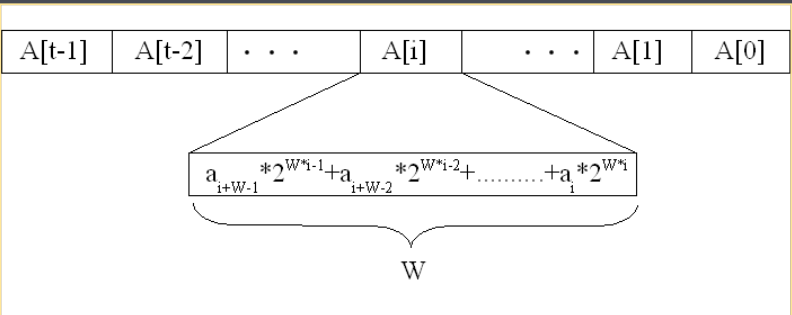
\includegraphics[width=0.8\textwidth]{figures/fig1-arrays-native-size}
    \centering
    \caption{Manuel Koschuch, Efficient Security for Mobile Communications Utilizing Elliptic Curves}
\end{figure}

\paragraph{Vorteile}

\begin{itemize}
    \item Die Langzahloperationen können auf Operationen auf nativer Wordgröße heruntergebrochen werden.
    \item Der zusätzliche Speicherbedarf ist maximal so groß wie ein natives Wort.
    \item Zugriff ist einfach und schnell.
    \item Vergleich von Langzahlen ist schnell und einfach.
    \item Verwendung von Langzahlen ist schnell und einfach.
\end{itemize}

\paragraph{Nachteile}

Operationen für diese Repräsentation sind nur bedingt parallelisierbar, es braucht hier eine carry-propagation.

%%% subsection %%%
\subsection{Arrays kleiner als die native Größe}

Sei wieder $W$ die native Wortgröße eines Prozessors und $x$ eine Zahl, deren Binärdarstellung $n$ bit benötigt. Jetzt verwenden wir das Array $A$, das 
$u = \lceil n/(W-k) \rceil$ Integers enthält, wobei $k$ ein für das entstehende Carry veranschlagter Speicher im Buffer ist.

\paragraph{Vorteile}

Hier haben wir ähnliche Vorteile wie bei Arrays in nativer Größe, zusätzlich haben wir Parallelisierbarkeit, weil zwei Worte addiert werden können, ohne dass carry-propagation 
notwendig wird.

\paragraph{Nachteile}

\begin{itemize}
    \item Potentiell höherer Speicherbedarf, da pro Wort $k$ Bit für carry frei bleiben
    \item Am Ende einer Rechnung muss carry sehr wohl propagiert werden (vgl. carry-save adders)
    \item Komplexere Behandlung der Elemente bei Rechnungen nötig, Konversion zu Beginn und am Ende einer Berechnung
\end{itemize}

%%% subsection %%%
\subsection*{Exkurs: Basisoperationen}

Seien $b, k \in \mathbb{N}$. Für jedes Stellensystem zur Basis $b$ gilt:

\paragraph{Multiplikation}

Eine Multiplikation mit dem Faktor $b^k$ entspricht einem Linksshift um $k$ Stellen. Beispiel:

\begin{align*}
    & 145 \cdot 10^2 = 14500 \\
    & 1101 \cdot 2^3 = 1101000
\end{align*}

\paragraph{Integer-Division}

Eine Integer-Division durch den Divisor $b^k$ entspricht einem Rechtshift um $k$ Stellen. Beispiel:

\begin{align*}
    & 7654 / 10^3 = 7 \\
    & 1110011101 / 2^5 = 11100
\end{align*}

\paragraph{Niederwertigste Stellen extrahieren}

Eine Modulo Operation mit Modul $b^k$ entspricht dem extrahieren der $k$ niederwertigsten Stellen. Beispiel:

\begin{align*}
    & 65432 \mod 10^3 = 432 \\
    & 111000101 \mod 2^4 = 0101
\end{align*}

\paragraph{Casting out nines}

Eine Modulo Operation mit Modul $b^k - 1$ entspricht dem teiler einer Zahl in $k$-stellige Blöcke, die dann aufsummiert werden. Beispiel:

$$34215 \mod (10^2 - 1) = 34215 \mod 99 = 3 + 42 + 15 = 60$$

%%% subsection %%%
\subsection{Modulo Reduktion}

Eine Moduloreduktion ist die Berechnung des kleinsten Repräsentanten einer Restklasse. Beispiel: die Zahl $17 \mod 5$ wird zu 2 reduziert.

\paragraph{Kriterien für den Einsatz}

Wie können wir feststellen, wann eine Moduloreduktion überhaupt notwendig ist? Grundsätzlich kann immer mit nichtreduzierten Zwischenergebnissen gerechnet werden. In der 
Praxis ist es aber sinnvoll, eine Reduktion anzuwenden, wenn das Zwischenergebnis mehr als 1 bit länger als der Modulus ist. Diese Bedingung ist über ein logisches Und 
vom MSW (most significant word) des Zwischenergebnisses und einer Bitmaske abhängig vom Modul einfach feststellbar.

\paragraph{Kosten von Langzahldivisionen}

Divisionen von Wörtern sind teure Operationen auf Computern. Langzahldivisionen sind sogar noch teurer, wie können wir den Aufwand verringern?  

Hierfür gibt es Berechnungen von Divisionsresten ohne (tatsächliche) Divisionen, nämlich 

\begin{itemize}
    \item Barrett Reduktion 
    \item Montgomery Multiplikation
\end{itemize}

\paragraph{Barrett Reduktion} 

Die Rechnung $(a\cdot b) / n$ wird berechnet als 

$$\frac{a\cdot b}{b^{2k-t}} \cdot \frac{b^{2k}}{n} \cdot \frac{1}{b^t},$$

wobei $b$ die Basis der Zahlendarstellung (in Digitalsystemen also 2) ist.

\paragraph{Montgomery Multiplikation}

Wenn $R$ eine Zweierpotenz ist und es ein $n'$ gibt, sodass $R \cdot R^{-1} - n\cdot n' = 1$, dann wird $a \cdot b \cdot R^{-1} \mod n$ berechnet mittels 

$$\frac{a\cdot b + (a \cdot b \cdot n'\mod R \cdot n)}{R}.$$

Hierfür benötigt es eine Hin- und Rücktransformation.

Diese Ansätze sind nur bei mehreren modularen Multiplikationen hintereinander sinnvoll, ansonsten ist der Transformationsoverhead zu groß.

\paragraph{Grundidee an Montgomery (todo)}

Ein $k$-faches von $n$ zum Produkt addieren, so dass die letzten $i$ Stellen 0 werden, und sich damit die
Division auf ein reines Shift beschränkt.  

Wie bestimmt sich $k$? \newline
Für die letzte Stelle $c$ muss (im Dezimalsystem) gelten: 

\begin{align*}
&c + k\cdot n = 0 \mod 10  \\
 &\Rightarrow c = -k \cdot n \mod 10 \\
 &\Rightarrow c \cdot -n^{-1} = k \mod 10
\end{align*}

Für die folgenden Stellen gilt analoges, nur mit entsprechendem Offset um $10^i$.  


De facto also:
Das Produkt mit dem negativen Inversen des Moduls multiplizieren (was ja gerade $n'$ ist), das ganze
modulo $R$ rechnen (was ja die neue Basis darstellt und sich auf ein Bitmaskieren der letzten Bits
beschränkt, wenn $R$ eine Zweierpotenz ist), mit dem Modulus multiplizieren und zum Produkt
addieren. Damit sind garantiert die letzten Bits 0 und können durch die Division einfach rausgeshiftet
werden.


\paragraph{Montgomery Beispiel (todo)}

Ein Beispiel im Dezimalsystem: Seien $a = 29, b = 48, n = 97$ und $R = 100$.

\textit{Hintransformation}:

\begin{align*}
    a' = a \cdot R \mod n = 29 \cdot 100 \mod 97 = 2900 \mod 97 = 87 \\
    b' = b \cdot R \mod n = 48 \cdot 100 \mod 97 = 4800 \mod 97 = 47
\end{align*}

\textit{Multiplikation}

Es gilt $a' \cdot b' = 87 \cdot 47 = 4089$. Jetzt versuchen wir die letzte und vorletzte Stelle zu 0 zu machen:

\begin{align*}
    4089 + 3\cdot n = 408\textbf{9} + 3 \cdot 97 = 408\textbf{9} \cdot 29\textbf{1} = 4380 \\
    43\textbf{8}0 + 60 \cdot n = 43\textbf{8}0 + 60 \cdot 97 = 43\textbf{8}0 + 85\textbf{2}0 = 10200
\end{align*}

Jetzt dividieren wir durch $R = 100$: $10200 / 100 = 102$.

\textit{Rücktransformation}

Wir berechnen 

$$102 \cdot R^{-1} \mod n = 102 \cdot 100^{-1} \mod 97 = 102 \cdot 65 \mod 97 = 34.$$

In der Gegenprobe haben wir $a \cdot b \mod n = 29 \cdot 48 \mod 97 = 34$.

Für die Abschätzung von Montgomery haben wir das 

\begin{lemma}
    Seien $a, b, n \in \mathbb{N}$, dann gilt 
    \begin{equation}
        \frac{a\cdot b + (a\cdot b\cdot n' \mod R) \cdot n}{R} < 2n.
    \end{equation}
\end{lemma}

\begin{proof} (Skizze):
    Wir wissen $a, b < n$ und $R > n$. Daher gilt $a\cdot b < n^2$. Weiters gilt immer $a\cdot b \cdot n' \mod R < R$. Deswegen gilt 

    $$\frac{a\cdot b + (a\cdot b\cdot n' \mod R) \cdot n}{R} < \frac{n^2 + R \cdot n}{R} = \frac{n^2}{R} + \frac{R\cdot n}{R} < n\cdot 1 + n = 2n.$$
\end{proof}

\paragraph{Mongomery Pseudocode (todo)}

Eine komplette Montgomery Multiplikation ist daher:

\begin{verbatim}
Input: a, b
Output: c = a*b mod n

t = a * b
c = t + (t*n' mod R)*n //mit R*R' - n*n' = 1
c = c/R
if (c > n)
    c = c - n
return c
\end{verbatim}

\begin{centering}
Monty(a,b) = a*b*R-1 mod n \\
Monty(a',b) = a*b mod n \\
Monty(a',b') = a'*b' mod n \\
Monty(a',1) = a mod n \\
Monty(a,R*R) = a' mod n 
\end{centering}

\section{Exponentiation}

Exponentiation ist eine häufige Operation, gerade bei RSA. Dabei hat der private Exponent häufig auch mindestens 1024 bits. 

\subsection{Square-and-Multiply}

Square-and-Multiply is die formalisierte Variante der ``Methode der wiederholten Quadrate''. Für jedes bit im Exponenten wird quadriert, wenn die bits 1 sind, dann 
auch multipliziert.

\begin{verbatim}
    Berechne m = c^d 

    m = 1
    for jedes Bit i in d, beginnend bei MSB, do 
        m = m*m 
        if (i = 1) then
            m = m \cdot c
    end 
    return m
\end{verbatim}

\paragraph{Beispiel} Berechnen von $x^12$ mittels Square-and-Multiply, dafür betrachten wir die Binärdarstellung $12 = b1100$:

\begin{verbatim}
    m = 1

    # i = 1, erstes bit, beginnend beim größten
    m = m * m = 1
    m = m * x = x

    # i = 1, zweites bit
    m = m * m = x^2
    m = m * x = x^3

    # i = 0, drittes bit
    m = m * m = x^6

    # i = 0, viertes bit
    m = m * m = x^12
\end{verbatim}

Hier fällt auf: je mehr \verb|1|er in der Binärdarstellung der Exponenten, desto größer ist unser Rechenaufwand.


\paragraph{Beispiel} Wir berechnen eine RSA Verschlüsselung mit $m = 7, p = 5$ und $q = 11$.

Wir haben $\varphi = 40$ und wählen $e = 3$, dann gilt $d = 27$ und $c = m^e \mod (p\cdot q) = 7^3 \mod 55 = 13$. Mittels Square-and-Multiply berechnen wir $m = c^d = 7$:

\begin{verbatim}
    27 = b11011

    m = 1

    # i = 1
    m = m * m = 1
    m = m * c = 13

    # i = 1 
    m = m * m = 13 * 13 mod 55 = 4
    m = m * c = 4 * 13 mod 55 = 52

    # i = 0
    m = m * m = 52 * 52 mod 55 = 9

    # i = 1
    m = m * m = 9 * 9 mod 55 = 26
    m = m * c = 26 * 13 mod 55 = 8 

    # i = 1 
    m = m * m = 8 * 8 mod 55 = 9
    m = m * c = 9 * 13 mod 55 = 7
\end{verbatim}

\subsection{NAF - Non-adjacent Form}

Im Durchschnitt braucht es für die Berechnung einer Exponentiation mit einem $n$-bit Exponenten:

\begin{itemize}
    \item $n/2$ Multiplikationen und
    \item $n$ Quadrierungen.
\end{itemize}

Unter Verwendung einer vorzeichenbehafteten Darstellung des Exponenten (mit $-1, 0$ und $1$) kann die Anzahl der Multiplikationen auf $n/3$ reduzier werden. In diesem Fall
wird die NAF de Exponenten berechnet.

\paragraph{Eigenschaften}

\begin{itemize}
    \item Sie ist eindeutig
    \item Sie hat die wenigsten Elemente ungleich 0 aller vorzeichenbehafteten Darstellungen
    \item Sie ist maximal $n+1$ bit lang 
    \item Es folgen niemals zwei Elemente ungleich 0 aufeinander 
    \item Sie hat durchschnittlich n/3 Elemente ungleich 0
\end{itemize}

Die Exponentiation ist ähnlich zu Square-and-Multiply, es wird nur vor der Berechnung die Inverse der Basis berechnet und in den Fällen, wo das Bit -1 ist, mit diesem 
Inversen statt mit der Basis multipliziert.

\paragraph{Beispiel} 

Wir berechnen die NAF von 12. Wir wissen $12 = b1100$, ihre NAF ist $10-100$, weil $12 = 2^4 - 2^2 = 16 - 4$.

\paragraph{Beispiel}

Wir berechnen die NAF von 7. Wir wissen $7 = 111$, die NAF ist $100-1$, weil $7 = 2^3 - 2^0 = 8 - 1$. Die Rechnung $x^7$ mittels NAF:

\begin{verbatim}
7 = 100-1 (NAF)

m = 1

# i = 1
m = m * m = 1
m = m * x = x

# i = 0
m = m * m = x^2 

# i = 0
m = m * m = x^4

# i = -1
m = m * m = x^8
m = m * x^{-1} = x^7
\end{verbatim}

\paragraph{Private Key bei RSA}

Privater Schlüssel d bei RSA üblicherweise signifikant länger als öffentlicher (1.024 Bits vs. 16 Bits). Problem: Entschlüsselung und Signaturgenerierung teuer. \\

Lösung: mittels CRT (Chinesicher Restsatz). Statt nur $d$ zu speichern, werden $p$, $q$, $dP$, $dQ$ und $qInv$ einmalig berechnet und gespeichert. Hierbei ist:

\begin{align*}
dP &= d \mod (p-1) \\
dQ &= d \mod (q-1) \\
qInv &= q^{-1} \mod p
\end{align*}

Die Entschlüsselung wird nicht als $m = c^d \mod n$ berechnet, sondern 

\begin{align*}
    m_1 &= c^{dP} \mod p \\
    m_2 &= c^{dQ} \mod q \\
    h &= qInv \cdot (m_1 - m_2) \mod p \\
    m &= m_2 + h\cdot q
\end{align*}

Dadurch sind die Exponenten statt 1024 nur noch ca 512 Bit lang.

\begin{verbatim}
    Private-Key: (4096 bit, 2 primes)

    modulus: //n (4.096 Bit)
    00:[…]:5a:ac:58:ff:66:e7

    publicExponent: //e (17 Bit) 
    65537 (0x10001)
    
    privateExponent: //d (4.096 Bit)
    00:a0:4d:a3:d7:f5:[…]:36:96:67:e5:c1

    prime1: //p (2.048 Bit)
    00:ed:22:[…]64:2c:07

    prime2: //q (2.048 Bit)
    00:d9:3f:[…]41:f6:21

    exponent1: //dP (2.048 Bit)
    00:cf:f1:[…]7f:be:ef

    exponent2: //dQ (2.048 Bit)
    58:f6:5d:[…]3d:c8:a1

    coefficient: //qInv (2.048 Bit)
    00:e4:01:[…]76:dd:61:b8
\end{verbatim}